\chapter{Resultados}

O problema proposto, o qual os testes serão realizados, se dá no próprio
ambiente de simulação de carros autônomos criado previamente. Com o objetivo de
medir o impacto do diferencial do NEAT — suas topologias aumentantes — serão
aplicados tr{\^e}s diferentes m{\'e}todos de treinamento:

\begin{enumerate}
	\item NEAT, proveniente do \textit{neat-python} pós parametrização, com topologia inicial m{\'i}nima;
	\item Neuroevolução, através da aplicação de um algoritmo genético sobre uma rede neural simples (sem topologias aumentantes);
	\item NEAT, com topologia inicial complexa.
\end{enumerate}

%% FIXME: generalidade?
Além destes, ser{\'a} tamb{\'e}m aplicado um teste de adapta{\c c}{\~a}o no
algoritmo, trocando a pista após o seu processo de treinamento com a finalidadede medir a
generalidade da tomada de decis{\~a}o.

Tais algoritmos trabalham de diferentes formas a encontrar valores de aptidão
para suas simulações. De modo a generalizar a classificação de resultados, foi
proposto a construção de um valor de pontua{\c c}{\~a}o atrelado à distância percorrida pelo
carro em sua execução.

Esta métrica pode vir a ser comparada entre métodos a fim de se encontrar
quanto tempo é necessário para se alcançar determinada \textit{fitness} e quanto é
alcançado após determinado tempo de execução decorrer.

Os resultados foram obtidos de duas diferentes formas: primeiramente
encontrando em que geração do algoritmo este consegue alcançar um valor de
\textit{fitness} mínimo necessário para que o carro execute uma volta completa pelo
trajeto, definindo assim quão rapidamente ele consegue alcançar uma resposta. 
E também a \textit{fitness} alcançada após determinado número de gerações ter sido executado. A
\autoref{fig_meta} ilustra dentro do ambiente de simulação o alvo a ser alcançado.

\begin{figure}[htb]
        \centering
        \caption{\label{fig_meta}Canto inferior esquerdo definido como meta a ser alcançada para obtenção de resultado.}
        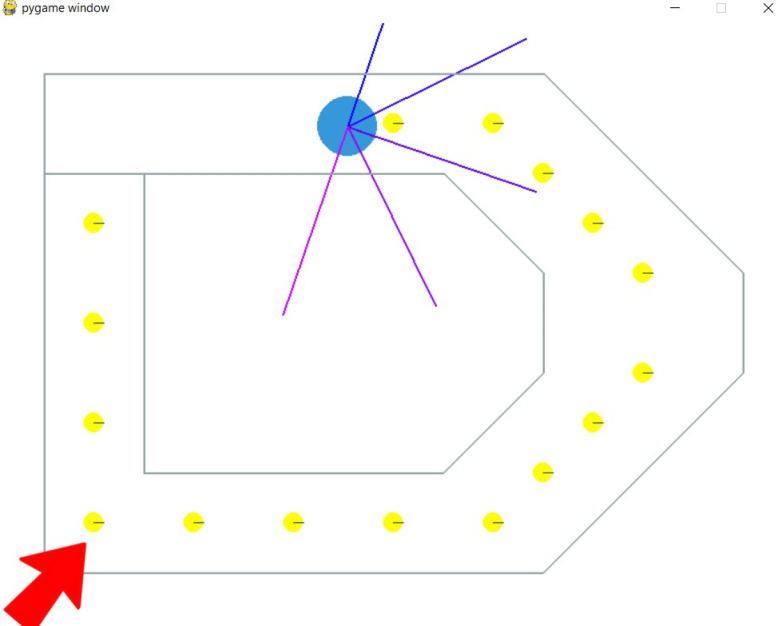
\includegraphics[width=0.5\textwidth]{images/meta.png}
        \legend{
                Fonte: Autoria Pr{\'o}pria.
        }
\end{figure}

A Rede Neural inicial é composta por 5 sensores que verificam e alimentam a
rede a cada movimento do carro e são elencados com os valores que vão de \textit{-5} até
\textit{-1}. Essas 5 entradas estão todas conectadas a cada uma das 3 saídas que indicam
a direção que o carro deve tomar, as saídas vão de \textit{0} até \textit{2}, sendo \textit{0} a indicação
de movimento à esquerda, \textit{1} à direita e 2 para frente. Cada conexão entre cada
sensor de entrada e cada nó de saída possui um peso específico que serve para a
geração do valor de saída. A estrutura indicada acima pode ser encontrada na
\autoref{fig_nn1}.

\begin{figure}[htb]
        \centering
        \caption{\label{fig_nn1}Organização da rede, com seus nós e conexões.}
        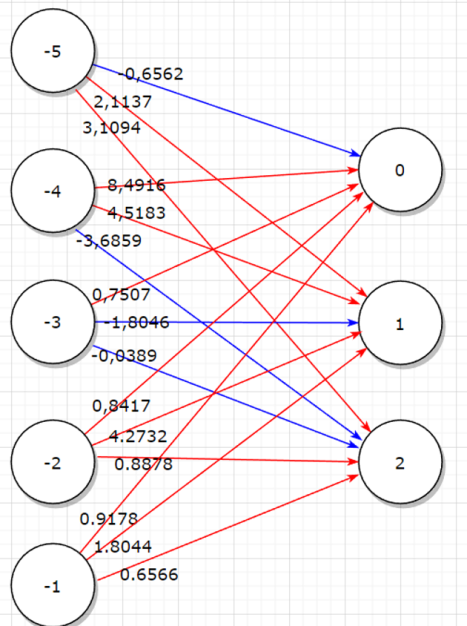
\includegraphics[width=0.4\textwidth]{images/nn1.png}
        \legend{
                Fonte: Autoria Pr{\'o}pria.
        }
\end{figure}

O processo de aprendizado de uma determinada rede veio a ser executado em um
ambiente de treinos, o qual, tratando-se do algoritmo NEAT, a topologia parte
de seu estado mais simples até possuir um determinado formato da qual é capaz
de finalizar o percurso, sendo tratada como a resposta ideal proposta. O
algoritmo de Neuroevolução também parte de seu estado mais simples até as
respostas desejadas neste ambiente.

\section{NEAT}

A simulação do treino para o algoritmo NEAT incorpora o aumento das topologias,
este pode vir a ser dado pela possibilidade de adições e subtrações de nós nas
camadas ocultas da rede e/ou remoção ou adição de conexões entre nós, fatores
observados nas redes dos resultados alcançados.

Foram realizadas três execuções com o objetivo de se alcançar a \textit{fitness} mínima
para que uma volta completa seja realizada em torno da pista, mensurado como
cerca de 16000 pontos de aptidão com 300 membros na população. Os resultados
com as respectivas gerações em que o cálculo foi alcançado se dão na \autoref{tabela_neat},
juntamente da topologia resultante em cada iteração.

\begin{table}[htb]
	\centering
    \caption{\label{tabela_neat}Resultados obtidos pelo NEAT até a meta de \textit{Fitness} ser alcançada.}
    \begin{tabular}{ccccc}
        \hline
		\textbf{Itera{\c c}{\~o}es} & \textbf{Topologia} & \textbf{Gera{\c c}{\~a}o} & \textbf{\textit{Fitness}} & \textbf{\textit{Fitness} média} \\ \hline
		1 & (3,13)  & 8   & 16379  & 3664 ± 2106   \\ \hline
		2 & (3,14)  & 3   & 16337  & 3285 ± 2165   \\ \hline
		3 & (4,13)  & 8   & 16336  & 3684 ± 2126   \\ \hline
    \end{tabular}
    \fonte{Autoria pr{\'o}pria.}
\end{table}

Como observável na \autoref{fig_nn2}, a terceira iteração obteve uma  topologia
a qual indica a existência de quatro nós e treze conexões totais, este nó
intermediário, inserido após um processo de mutação, serve como uma conexão na
camada oculta entre a entrada \textit{-2} e as saídas \textit{1} e \textit{2}. Além desta mudança, a
topologia também sofreu alterações com a remoção da conexão entre a entrada \textit{-3}
e saída \textit{0}, julgada pelo algoritmo como uma melhoria para o desempenho durante
suas mutações e cruzamentos.

\begin{figure}[htb]
        \centering
        \caption{\label{fig_nn2}Rede neural da Iteração 3 de treinos do algoritmo NEAT, com uma conexão excluída e um nó adicional na camada oculta.}
        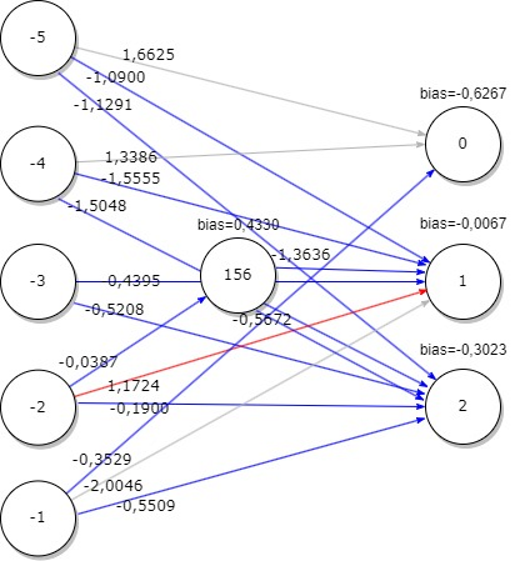
\includegraphics[width=0.4\textwidth]{images/nn2.png}
        \legend{
                Fonte: Autoria Pr{\'o}pria.
        }
\end{figure}

A segunda bateria de treinos englobava a execução do algoritmo até sua 10ª
geração, e a comparação dos resultados obtidos até então. Seus resultados são
observáveis na \autoref{tabela_neat_10}.

\begin{table}[htb]
	\centering
    \caption{\label{tabela_neat_10}Resultados obtidos pelo NEAT após a execução de 10 gerações.}
    \begin{tabular}{ccccc}
        \hline
		\textbf{Itera{\c c}{\~o}es} & \textbf{Topologia} & \textbf{Gera{\c c}{\~a}o} & \textbf{\textit{Fitness}} & \textbf{\textit{Fitness} média} \\ \hline
		1 & (4,9)   & 10  & 16383  & 3191 ± 2524   \\ \hline
		2 & (3,12)  & 10  & 18528  & 3847 ± 1997   \\ \hline
		3 & (4,15)  & 10  & 14199  & 3569 ± 1903   \\ \hline
    \end{tabular}
    \fonte{Autoria pr{\'o}pria.}
\end{table}

Observando a topologia da iteração de número 2, é possível verificar que esta
que obteve a maior \textit{fitness} em 10 gera{\c c}{\~o}es, identificou como
uma melhora no resultado a quebra da conexão entre a entrada \textit{-5} e a saída \textit{0} e a
entrada \textit{-1} e saída \textit{2}, como observável na \autoref{fig_nn3}.

\begin{figure}[htb]
        \centering
        \caption{\label{fig_nn3}Rede neural da Iteração 2 de treinos do algoritmo NEAT, com duas conexões excluídas e uma desativada.}
        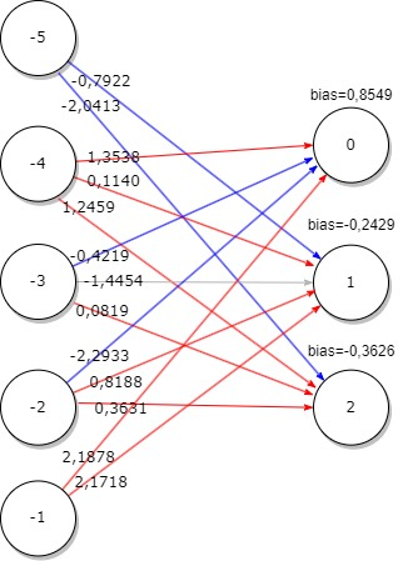
\includegraphics[width=0.4\textwidth]{images/nn3.png}
        \legend{
                Fonte: Autoria Pr{\'o}pria.
        }
\end{figure}

\section{Neuroevolu{\c c}{\~a}o}

Para a simulação de um algoritmo básico de Neuroevolução sem a etapa de aumento
de topologias, se fez uso da mesma estrutura utilizada anteriormente pelo NEAT,
porém sem a possibilidade de haver adições ou subtrações de nós (nas camadas
ocultas) ou conexões (entre entradas, nós e saídas).

Como apresentado na \autoref{tabela_ne}, o algoritmo foi executado três vezes com
diferentes valores para \textit{fitness} alcançada e em que geração estas se deram,
considerando uma população de 300 integrantes.

A coluna de topologia não se faz necessária considerando que este, por se
tratar de um algoritmo simples de neuroevolução, possui suas tomadas de
decisões realizadas apenas na pesagem de suas arestas, sem alterações de
topologia durante a execução.

\begin{table}[htb]
	\centering
    \caption{\label{tabela_ne}Resultados obtidos em suas respectivas gerações após execução do algoritmo de Neuroevolução.}
    \begin{tabular}{cccc}
        \hline
		\textbf{Itera{\c c}{\~o}es} & \textbf{Gera{\c c}{\~a}o} & \textbf{\textit{Fitness}} & \textbf{\textit{Fitness} média} \\ \hline
		1 & 3   & 16345  & 3354 ± 2138   \\ \hline
		2 & 12  & 16373  & 3839 ± 1930   \\ \hline
		3 & 12  & 16382  & 3788 ± 2298   \\ \hline
    \end{tabular}
    \fonte{Autoria pr{\'o}pria.}
\end{table}

A rede neural referente à iteração que alcançou o resultado mais rapidamente
pode ser expressa na \autoref{fig_nn4}, com suas devidas conexões e pesos.

\begin{figure}[htb]
        \centering
        \caption{\label{fig_nn4}Rede neural da Iteração 1 de treinos do algoritmo de Neuroevolução.}
        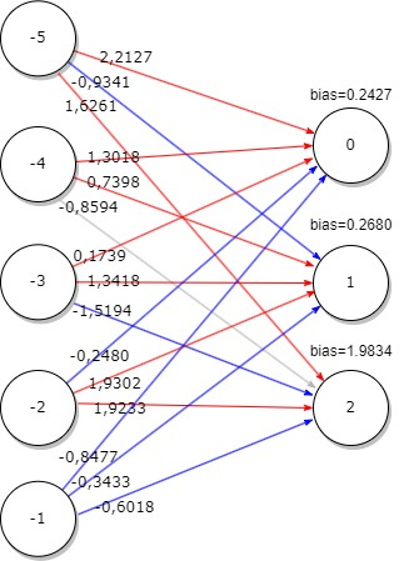
\includegraphics[width=0.4\textwidth]{images/nn4.png}
        \legend{
                Fonte: Autoria Pr{\'o}pria.
        }
\end{figure}

A \autoref{tabela_ne_10} ilustra os resultados obtidos para o algoritmo de
Neuroevolução considerando três execuções até a décima geração, com a \textit{fitness}
média e máxima alcançadas dentro da população de 300 integrantes para cada
iteração. Do mesmo modo, a rede neural com o resultado da iteração de melhor
resultado pode ser expressa na \autoref{fig_nn5}, com suas devidas conexões e
pesos.

\begin{table}[htb]
	\centering
    \caption{\label{tabela_ne_10}Resultados obtidos até a décima geração após execução do algoritmo de Neuroevolução.}
    \begin{tabular}{cccc}
        \hline
		\textbf{Itera{\c c}{\~o}es} & \textbf{Gera{\c c}{\~a}o} & \textbf{\textit{Fitness}} & \textbf{\textit{Fitness} média} \\ \hline
		1 & 10  & 16356  & 3754 ± 2159   \\ \hline
		2 & 10  & 19596  & 3923 ± 2101   \\ \hline
		3 & 10  & 16335  & 3767 ± 1966   \\ \hline
    \end{tabular}
    \fonte{Autoria pr{\'o}pria.}
\end{table}

\begin{figure}[htb]
        \centering
        \caption{\label{fig_nn5}Rede neural da Iteração 2 após 10 gerações de treinos do algoritmo de Neuroevolução.}
        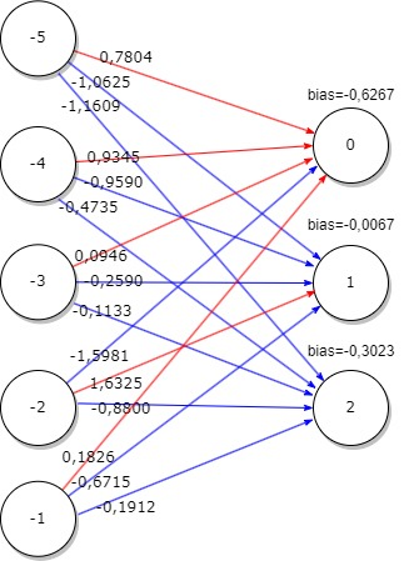
\includegraphics[width=0.4\textwidth]{images/nn5.png}
        \legend{
                Fonte: Autoria Pr{\'o}pria.
        }
\end{figure}

\section{NEAT com Topologia Inicial Complexa}

\begin{table}[htb]
	\centering
    \caption{\label{tabela_neatc}Resultados obtidos pelo NEAT com topologia inicial complexa até a meta de \textit{Fitness} ser alcançada.}
    \begin{tabular}{ccccc}
        \hline
		\textbf{Itera{\c c}{\~o}es} & \textbf{Topologia} & \textbf{Gera{\c c}{\~a}o} & \textbf{\textit{Fitness}} & \textbf{\textit{Fitness} média} \\ \hline
		1 & (8,40)  & 23  & 16339  & 1010 ± 2314   \\ \hline
		2 & (8,39)  & 2   & 16429  & 1220 ± 1992   \\ \hline
		3 & (8,39)  & 23  & 16319  & 1379 ± 2785   \\ \hline
    \end{tabular}
    \fonte{Autoria pr{\'o}pria.}
\end{table}

Pode-se observar a elevada vari{\^a}ncia dos resultados — indicando uma
dificuldade do algoritmo evitar os m{\'a}ximos locais com essa quantidade
elevada de n{\'o}s. Outro ponto observável é a conservação da topologia — o algoritmo
teve melhor performance ao evitar a remo{\c c}{\~a}o de nós, e removendo
somente uma ou at{\'e} nenhuma das conex{\~o}es.

Tamb{\'e}m percebe-se a occor{\'e}ncia m{\'u}ltipla da gera{\c c}{\~a}o 32 —
isso se d{\'a} pelo funcionamento interno do \textit{neat-python}, em que a
partir da gera{\c c}{\~a}o 20, come{\c c}a-se a eliminar as esp{\'e}cies
\textit{estagnadas}, ou seja, indiv{\'i}duos que estavam sendo utilizados pela
possibilidade de haver caracter{\'i}sticas {\'u}teis, por{\'e}m n{\~a} deram
resultado. Com essa popula{\c c}{\~a}o removida, o algoritmo consegue assim
atingir o objetivo em algumas gera{\c c}{\~o}es.

\section{Adapta{\c c}{\~a}o a ambiente de testes}

%% FIXME: generalidade?
O ambiente de teste foi estruturado como mostrado na \autoref{fig_teste}, de
modo semelhante ao ambiente de treino, por{\'e}m, com altera{\c c}{\~o}es no
percurso de modo a testar a generalidade da solu{\c c}{\~a}o encontrada. Os
algoritmos foram executados at{\'e} a meta previamente determinada (em torno de
16000 de \textit{fitness}) e no fim do treinamento foram expostos ao novo
ambiente, tendo a medida de sua dist{\^a}ncia percorrida at{\'e} a primeira
colis{\~a}o.

\begin{figure}[htb]
        \centering
        \caption{\label{fig_teste}Percurso alternativo de teste.}
        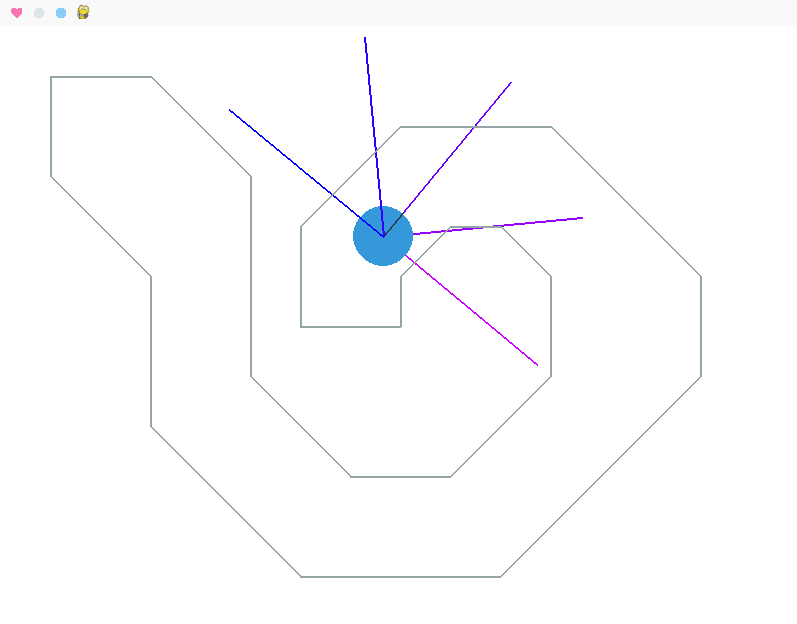
\includegraphics[width=0.5\textwidth]{images/teste.png}
        \legend{
                Fonte: Autoria Pr{\'o}pria.
        }
\end{figure}

Uma medida de sucesso pode ser considerada o caminho completo ser percorrido, o que foi
medido como sendo um número próximo de 1200 de dist{\^a}ncia.

Aplicando essa t{\'e}cnica com o algoritmo NEAT parametrizado, se obteve os
resultados apresentados na \autoref{tabela_teste_neat}.

\begin{table}[htb]
	\centering
	\caption{\label{tabela_teste_neat}Resultados obtidos pelo NEAT sendo exposto a um ambiente diferente ap{\'o}s a meta de \textit{Fitness} ser alcançada.}
    \begin{tabular}{ccccc}
        \hline
		\textbf{Itera{\c c}{\~o}es} & \textbf{Topologia} & \textbf{Gera{\c c}{\~a}o} & \textbf{\textit{Fitness}} & \textbf{Resultado do teste} \\ \hline
		1 & (3,13)  & 9   & 16384  & 1386   \\ \hline
		2 & (4,12)  & 8   & 16412  & 134    \\ \hline
		3 & (3,12)  & 7   & 16348  & 250    \\ \hline
    \end{tabular}
    \fonte{Autoria pr{\'o}pria.}
\end{table}

Aplicando o mesmo para a neuroevolu{\c c}{\~a}o sem topologias vari{\'a}veis,
se obteve os resultados apresentados na \autoref{tabela_teste_ne}.

\begin{table}[htb]
	\centering
	\caption{\label{tabela_teste_ne}Resultados obtidos pela neuroevolu{\c c}{\~a}o sem topologia vari{\'a}vel sendo exposta a um ambiente diferente ap{\'o}s a meta de \textit{Fitness} ser alcançada.}
    \begin{tabular}{ccccc}
        \hline
		\textbf{Itera{\c c}{\~o}es} & \textbf{Topologia} & \textbf{Gera{\c c}{\~a}o} & \textbf{\textit{Fitness}} & \textbf{Resultado do teste} \\ \hline
		1 & (3,15)  & 8   & 16357  & 167  \\ \hline
		2 & (3,15)  & 16  & 16354  & 16   \\ \hline
		3 & (3,15)  & 4   & 16319  & 22   \\ \hline
    \end{tabular}
    \fonte{Autoria pr{\'o}pria.}
\end{table}

Por fimm aplicando o mesmo para o NEAT com topologia complexa inicial, se obteve
os resultados apresentados na \autoref{tabela_teste_neatc}.

\begin{table}[htb]
	\centering
	\caption{\label{tabela_teste_neatc}Resultados obtidos pelo NEAT com topologia inicial complexa sendo exposto a um ambiente diferente ap{\'o}s a meta de \textit{Fitness} ser alcançada.}
    \begin{tabular}{ccccc}
        \hline
		\textbf{Itera{\c c}{\~o}es} & \textbf{Topologia} & \textbf{Gera{\c c}{\~a}o} & \textbf{\textit{Fitness}} & \textbf{Resultado do teste} \\ \hline
		1 & (8,39)  & 23  & 16390  & 1129   \\ \hline
		2 & (8,38)  & 22  & 16397  & 180   \\ \hline
		3 & (8,38)  & 2   & 16328  & 133   \\ \hline
    \end{tabular}
    \fonte{Autoria pr{\'o}pria.}
\end{table}

\section{Análise de Resultados}

Comparando os dois primeiros cen{\'a}rios, a
neuroevolu{\c c}{\~a}o chegou próxima da
performance do NEAT, principalmente nos
cen{\'a}rios a longo prazo (10 gera{\c
c}{\~o}es), em que a neuroevolu{\c c}{\~a}o
tende a alcan{\c c}ar resultados
melhores que o NEAT. Enquanto isso pode ser
atribuido {\`a} simplicidade do problema
utilizado, observando os resultados de adapta{\c
c}{\~a}o em um ambiente alternativo para teste, o
NEAT chegou em uma solu{\c c}{\~a}o mais
generalizada do que a neuroevolu{\c c}{\~a}o,
conseguindo at{\'e} mesmo completar o percurso.

Analisando o cen{\'a}rio com a topologia
complexa, pode-se observar uma dificuldade do
algoritmo a enfrentar m{\'a}ximos locais,
levando diversas gera{\c c}{\~o}es para
ultrapass{\'a}-los. Tamb{\'e}m foi possível
observado a perda de performance imediata nas
altera{\c c}{\~o}es de topologia, fazendo com
que o algoritmo mantesse sua topologia muito
proxima da original - o que pode ter acarretado
o problema de m{\'a}ximos locais. Um ponto
positivo se dá no fato da topologia complexa ter levado a
solu{\c c}{\~o}es mais inteligentes em respeito
a adapta{\c c}{\~a}o para o ambiente de teste,
chegando pr{\'o}ximo do final do percurso.

No geral, a performance dos algoritmos na
adapta{\c c}{\~a}o para a troca do ambiente,
enquanto poss{\'i}vel, foi inconsistente.
